\documentclass[10pt,a4paper]{article}
\usepackage{blindtext}
\usepackage{subcaption}
\usepackage{graphicx}
\usepackage{tikz}
\usepackage{amssymb}
\usepackage{caption}
\usepackage{amsmath}
\usepackage{circuitikz}
\usepackage{hyperref}
\usepackage{amssymb}
\usepackage{amsmath}
\usepackage{listings}

\lstset{
    inputencoding=utf8,
    extendedchars=true,
    literate={á}{{\'a}}1 {é}{{\'e}}1 {í}{{\'i}}1 {ó}{{\'o}}1 {ú}{{\'u}}1 {ñ}{{\~n}}1 {Á}{{\'A}}1 {É}{{\'E}}1 {Í}{{\'I}}1 {Ó}{{\'O}}1 {Ú}{{\'U}}1 {Ñ}{{\~N}}1
}
\usepackage[spanish,activeacute,es-tabla]{babel}
\usepackage[utf8]{inputenc}
\usepackage{ifthen}
\usepackage{listings}
\usepackage{dsfont}
\usepackage{subcaption}
\usepackage{amsmath}
\usepackage[strict]{changepage}
\usepackage[top=1cm,bottom=2cm,left=1cm,right=1cm]{geometry}%
\usepackage{color}%
\newcommand{\tocarEspacios}{%
	\addtolength{\leftskip}{3em}%
	\setlength{\parindent}{0em}%
}

% Especificacion de procs

\newcommand{\In}{\textsf{in }}
\newcommand{\Out}{\textsf{out }}
\newcommand{\Inout}{\textsf{inout }}

\newcommand{\encabezadoDeProc}[4]{%
	% Ponemos la palabrita problema en tt
	%  \noindent%
	{\normalfont\bfseries\ttfamily proc}%
	% Ponemos el nombre del problema
	\ %
	{\normalfont\ttfamily #2}%
	\
	% Ponemos los parametros
	(#3)%
	\ifthenelse{\equal{#4}{}}{}{%
		% Por ultimo, va el tipo del resultado
		\ : #4}
}

\newenvironment{proc}[4][res]{%
	
	% El parametro 1 (opcional) es el nombre del resultado
	% El parametro 2 es el nombre del problema
	% El parametro 3 son los parametros
	% El parametro 4 es el tipo del resultado
	% Preambulo del ambiente problema
	% Tenemos que definir los comandos requiere, asegura, modifica y aux
	\newcommand{\requiere}[2][]{%
		{\normalfont\bfseries\ttfamily requiere}%
		\ifthenelse{\equal{##1}{}}{}{\ {\normalfont\ttfamily ##1} :}\ %
		\{\ensuremath{##2}\}%
		{\normalfont\bfseries\,\par}%
	}
	\newcommand{\asegura}[2][]{%
		{\normalfont\bfseries\ttfamily asegura}%
		\ifthenelse{\equal{##1}{}}{}{\ {\normalfont\ttfamily ##1} :}\
		\{\ensuremath{##2}\}%
		{\normalfont\bfseries\,\par}%
	}
	\renewcommand{\aux}[4]{%
		{\normalfont\bfseries\ttfamily aux\ }%
		{\normalfont\ttfamily ##1}%
		\ifthenelse{\equal{##2}{}}{}{\ (##2)}\ : ##3\, = \ensuremath{##4}%
		{\normalfont\bfseries\,;\par}%
	}
	\renewcommand{\pred}[3]{%
		{\normalfont\bfseries\ttfamily pred }%
		{\normalfont\ttfamily ##1}%
		\ifthenelse{\equal{##2}{}}{}{\ (##2) }%
		\{%
		\begin{adjustwidth}{+5em}{}
			\ensuremath{##3}
		\end{adjustwidth}
		\}%
		{\normalfont\bfseries\,\par}%
	}
	
	\newcommand{\res}{#1}
	\vspace{1ex}
	\noindent
	\encabezadoDeProc{#1}{#2}{#3}{#4}
	% Abrimos la llave
	\par%
	\tocarEspacios
}
{
	% Cerramos la llave
	\vspace{1ex}
}

\newcommand{\aux}[4]{%
	{\normalfont\bfseries\ttfamily\noindent aux\ }%
	{\normalfont\ttfamily #1}%
	\ifthenelse{\equal{#2}{}}{}{\ (#2)}\ : #3\, = \ensuremath{#4}%
	{\normalfont\bfseries\,;\par}%
}

\newcommand{\pred}[3]{%
	{\normalfont\bfseries\ttfamily\noindent pred }%
	{\normalfont\ttfamily #1}%
	\ifthenelse{\equal{#2}{}}{}{\ (#2) }%
	\{%
	\begin{adjustwidth}{+2em}{}
		\ensuremath{#3}
	\end{adjustwidth}
	\}%
	{\normalfont\bfseries\,\par}%
}

% Tipos

\newcommand{\nat}{\ensuremath{\mathds{N}}}
\newcommand{\ent}{\ensuremath{\mathds{Z}}}
\newcommand{\float}{\ensuremath{\mathds{R}}}
\newcommand{\bool}{\ensuremath{\mathsf{Bool}}}
\newcommand{\cha}{\ensuremath{\mathsf{Char}}}
\newcommand{\str}{\ensuremath{\mathsf{String}}}

% Logica

\newcommand{\True}{\ensuremath{\mathrm{true}}}
\newcommand{\False}{\ensuremath{\mathrm{false}}}
\newcommand{\Then}{\ensuremath{\rightarrow}}
\newcommand{\Iff}{\ensuremath{\leftrightarrow}}
\newcommand{\implica}{\ensuremath{\longrightarrow}}
\newcommand{\IfThenElse}[3]{\ensuremath{\mathsf{if}\ #1\ \mathsf{then}\ #2\ \mathsf{else}\ #3\ \mathsf{fi}}}
\newcommand{\yLuego}{\land _L}
\newcommand{\oLuego}{\lor _L}
\newcommand{\implicaLuego}{\implica _L}

\newcommand{\cuantificador}[5]{%
	\ensuremath{(#2 #3: #4)\ (%
		\ifthenelse{\equal{#1}{unalinea}}{
			#5
		}{
			$ % exiting math mode
			\begin{adjustwidth}{+2em}{}
				$#5$%
			\end{adjustwidth}%
			$ % entering math mode
		}
		)}
}

\newcommand{\existe}[4][]{%
	\cuantificador{#1}{\exists}{#2}{#3}{#4}
}
\newcommand{\paraTodo}[4][]{%
	\cuantificador{#1}{\forall}{#2}{#3}{#4}
}

%listas

\newcommand{\TLista}[1]{\ensuremath{seq \langle #1\rangle}}
\newcommand{\lvacia}{\ensuremath{[\ ]}}
\newcommand{\lv}{\ensuremath{[\ ]}}
\newcommand{\longitud}[1]{\ensuremath{|#1|}}
\newcommand{\cons}[1]{\ensuremath{\mathsf{addFirst}}(#1)}
\newcommand{\indice}[1]{\ensuremath{\mathsf{indice}}(#1)}
\newcommand{\conc}[1]{\ensuremath{\mathsf{concat}}(#1)}
\newcommand{\cab}[1]{\ensuremath{\mathsf{head}}(#1)}
\newcommand{\cola}[1]{\ensuremath{\mathsf{tail}}(#1)}
\newcommand{\sub}[1]{\ensuremath{\mathsf{subseq}}(#1)}
\newcommand{\en}[1]{\ensuremath{\mathsf{en}}(#1)}
\newcommand{\cuenta}[2]{\mathsf{cuenta}\ensuremath{(#1, #2)}}
\newcommand{\suma}[1]{\mathsf{suma}(#1)}
\newcommand{\twodots}{\ensuremath{\mathrm{..}}}
\newcommand{\masmas}{\ensuremath{++}}
\newcommand{\matriz}[1]{\TLista{\TLista{#1}}}
\newcommand{\seqchar}{\TLista{\cha}}

\renewcommand{\lstlistingname}{Código}
\lstset{% general command to set parameter(s)
	language=Java,
	morekeywords={endif, endwhile, skip},
	basewidth={0.47em,0.40em},
	columns=fixed, fontadjust, resetmargins, xrightmargin=5pt, xleftmargin=15pt,
	flexiblecolumns=false, tabsize=4, breaklines, breakatwhitespace=false, extendedchars=true,
	numbers=left, numberstyle=\tiny, stepnumber=1, numbersep=9pt,
	frame=l, framesep=3pt,
	captionpos=b,
}

\newcommand{\notimplies}{\;\not\!\!\!\implies}
\title{Paradigmas de Lenguajes de Programación}
\author{Tomás Agustín Hernández}
\date{}

\begin{document}
\maketitle

\begin{figure}[b]
    \centering
    \begin{tikzpicture}[remember picture,overlay]
        \node[anchor=south east, inner sep=0pt, xshift=-1cm, yshift=2cm] at (current page.south east) {
            \begin{minipage}[b]{0.5\textwidth}
                
\includegraphics[width=\linewidth]{logo_uba.jpg}
                \label{fig:bottom}
            \end{minipage}
        };
    \end{tikzpicture}
\end{figure}

\newpage
\section*{Programación Funcional}
Consiste en definir funciones y aplicarlas para procesar información. \\
Las funciones son verdaderamente funciones (parciales): 
\begin{itemize}
    \item Aplicar una función no tiene efectos secundarios.
    \item A una misma entrada le corresponde siempre la misma salida.
    \item Las estructuras de datos son inmutables.
\end{itemize}
Las funciones, además son datos como cualquier otro:
\begin{itemize}
    \item Se pueden pasar como parámetros.
    \item Se pueden devolver como resultados.
    \item Pueden formar parte de estructuras de datos. Ej.: Un árbol binario que en sus nodos hay funciones.
\end{itemize}
\subsection*{Expresiones}
Son secuencias de símbolos que sirven para representar datos, funciones, y funciones aplicadas a los datos. \\
Una expresión puede ser:
\begin{itemize}
    \item Un constructor: True, False, [], (:), 0, 1, 2. 
    \begin{itemize}
        \item Type Constructor: Es un constructor que se utiliza para crear un nuevo tipo.
        \item Data Constructor: Se utiliza para crear valores de ese tipo.
        \item Ej.: $data \ Color \ = \ Rojo \ | \ Verde \ | \ Azul$. Azul es un \textbf{data constructor} pues nos permite crear valores del tipo Color mientras que el Type Constructor es Color.
        \item Ej.: $data \ Complejo \ = \ C \ Float \ Float $. C es una función que recibe dos Float y es un constructor de Complejo.
    \end{itemize}
    \item Una variable: longitud, ordenar, x, xs (+), (*). 
    \item La aplicación de una expresión a otra: ordenar lista, not True, (+) 1. 
\end{itemize}
\subsection*{Función Parcialmente Aplicada}
Una función parcialmente aplicada es una función a las cuales se llama otra función pero no se le proporcionan todos los argumentos. \\
Ahora, es importante que para que esta función parcialmente aplicada tenga sentido, se le manden todos los parámetros. \\
Es una especie de $ a \rightarrow b$
Ej.: 
\begin{lstlisting}
    add :: Int -> Int -> Int
    add x y = x + y

    add5 :: Int -> Int
    add5 = add 5

    add5 es una función que ejecuta la función parcial add pues le manda solo un parámetro y necesita dos.
   
\end{lstlisting}
Una buena pregunta entonces es ¿pero por qué es una función parcial add 5? Pues hay una función add5 que la implementa sin pasarle todos los parámetros directamente explícitamente.
\begin{lstlisting}
    add5 3 -> Este 3 llega como "y" a add

    add5 = add 5 
    add = 5 + y
    add = 5 + 3
    add = 8 

\end{lstlisting}

\subsection*{Aplicación de Expresiones}
Es asociativa hacia la izquierda:
\begin{itemize}
    \item $ f \ x \ y \equiv \ (f \ x) \ y $
    \item $ ((((f \ a) \ b) \ c) \ d)$: Primero calcula el resultado que devuelve la expresión f enviando el valor de a. Nótese que la ídea seria que (f a) devuelva una expresión del tipo función pues luego le pasamos otro parámetro (b).
\end{itemize}
\subsection*{Construyendo una lista paso a paso con constructores}
Ej.: ¿Como construimos la lista [1, 2] utilizando constructores?
\begin{itemize}
    \item Lo primero que necesitamos, es un constructor de listas. Para eso tenemos la expresión (:). Recordando que la aplicación de expresiones es asociativo a izquierda.
    \item Veamos su tipo desde GHCI $(:) \ :: \ a \ -> \ [a] -> \ [a]$.
    \item Necesitamos enviarle un valor de tipo a, una lista y como resultado, la operación (:) devuelve una lista. 
    \item Preguntemos lo siguiente: ¿Con ((:) 1) nos basta para agregar a una lista? No, porque no estamos cumpliendo el tipado del constructor. Si quisieramos una lista con solamente el 1 si bastaría, pero acá también queremos el 2.
    \item Entonces, comenzamos aplicando la expresión (:) con el número 2, y ahí sí enviamos como segundo parámetro una lista vacía (que da como resultado) una lista vacía.
    \item (((:) 2) []) = [2]
    \item Por último, ((:) 1) [2] también cumple el tipo pues nos quedaría ((:) 1) [2] = [1, 2]
\end{itemize}
¿Y si quisieramos construir 1, 2, 3, 4? Recordemos la asociatividad a la izquierda, pero a la hora de querer utilizar una expresión, hay que cumplir el tipado. Hasta que ese tipado no se cumpla, Haskell tratará de resolver la expresión más profunda para ver si reduciendo cumple el tipo. \\
\[((:) 1) \ (((:) \ 4)(((:) \ 2) (((:) \ 3) \ [])))\] \\
Esto lo podemos ver como $a \rightarrow (b \rightarrow (c \rightarrow (d))) $ pues para conocer a, necesitamos construir la lista de la derecha, para conocer a b necesitamos la lista de la derecha, para conocer a c necesitamos la lista de d, y d inicializa la lista vacía. Esto es importantísimo porque claramente no podríamos usar (:) 1 sin una lista. Entonces Haskell evalúa todo lo de la derecha hasta que obtenga una lista. Si no se obtuviera una lista, sería inválido. \\
\section*{Polimorfismo}
Sucede en aquellas expresiones que tienen más de un tipo. 
\begin{itemize}
    \item $ id \ :: \ a \rightarrow a $
    \item $(:) :: a \rightarrow [a] \rightarrow [a]$
    \item $fst :: (a, b) \rightarrow a$
    \item $cargarStringArray :: String -> [] \rightarrow [String]$. No es una expresión Polimórfica.
\end{itemize}
\textbf{Nota}: Es importante que si tenemos 2 parámetros de tipo a significa que los dos parámetros deben ser de ese tipo. Si tenemos 2 parámetros uno de tipo a y uno de b podría suceder que sean diferentes pero puede que sean el mismo. 
\section*{Modelo de Cómputo (cálculo de valores)}
Dada una expresión, se computa su valor usando las ecuaciones siempre y cuando estén bien tipadas. \\
\textbf{Importante}: Que una expresión se cumpla el tipado, no significa que devuelva un valor.
\begin{itemize}
    \item $sumarUno :: a -> a$: No falla nunca.
    \item $division :: a -> b$: Falla si b = 0. Esto nos demuestra que aunque los parámetros estén bien tipados, podemos tener indefiniciones.
\end{itemize}
\subsection*{¿Cómo está dado un programa en Funcional?}
Un programa funcional está dado por un conjunto de \textbf{ecuaciones orientadas}. Se les llama de esta forma pues del \textbf{lado izquierdo está lo que define y del lado derecho la definición} (o expresión que produce el valor)
Una ecuación e1 = e2 se interpreta desde dos puntos de vista
\begin{itemize}
    \item \textbf{Denotacional}: Declara que e1 y e2 tienen el mismo significado. 
    \begin{itemize}
        \item "\textbf{Denotan} lo mismo"
    \end{itemize}
    \item \textbf{Operacional}: Computar el valor de e1 se reduce a computar el valor de e2.
    \begin{itemize}
        \item "\textbf{Operan} de la misma forma"
    \end{itemize}
\end{itemize}
\subsection*{¿Cómo es el lado izquierdo de una ecuación orientada?}
No es una expresión arbitraria. Debe ser una función aplicada a \textbf{patrones}. \\
Un patrón puede ser: 
\begin{itemize}
    \item Una variable: a, b, c.
    \item Un comodin: \textunderscore. 
    \item Un constructor aplicado a patrones: Recordemos que un constructor sería algo que construye un tipo. 
    \begin{itemize}
        \item True, False, 1, etc.
    \end{itemize}
\end{itemize}
\textbf{Importante}: El lado izquierdo NO debe contener variables repetidas. \\
Ej.: $iguales \ x \ x \ = \ True$ es una expresión mal formada. Esto pues dos valores que pueden ser diferentes, no pueden caer en la misma variable. \\
Ej.: $predecesor \ (n+1) \ = \ n$ también está mal formada porque estamos haciendo un cálculo del lado izquierdo, y recordemos que del lado izquierdo solo hay definiciones. Del lado derecho se hacen los cómputos o cálculo de los valores.
\subsection*{¿Cómo evalúamos las expresiones?}
\begin{itemize}
    \item Buscamos la subexpresión más externa que coincida con el lado izquierdo de una ecuación.
    \item Reemplazar la subexpresión que coincide con el lado izquierdo de la ecuación por la expresión correspondiente al lado derecho.
    \item Continuar evaluando la expresión resultante.
\end{itemize}
\subsection*{¿Cuando se detiene la evaluación de una expresión?}
\begin{itemize}
    \item Cuando el programa estalla (da error).
    \item Cuando la expresión es una función \textbf{parcialmente aplicada}. ¿que seria esto? 
    \item La expresión es un constructor o un constructor aplicado. Ej.: True, (:) 1, [1, 2, 3]. 
    \begin{itemize}
        \item Yo lo veo como algo más del tipo: una fórmula atómica o algo irreducible.
    \end{itemize}
\end{itemize}
\section*{Recordando Haskell}
Para ejecutar un archivo hay que instalar GHCI. Una vez instalado, nos paramos en la terminal en el directorio donde está el archivo que queremos ejecutar. 
\begin{itemize}
    \item Cargar archivo: :l nombreArchivo
    \item Ver tipo: :type tipo 
    \item Ejecutar funcion: funcion parametro1 parametro2...
    \item Recargar archivo: :r
    \item Si necesitamos hacer cálculos para mandar un parámetro, usar paréntesis: Ej.: otherwise = n * factorial(n-1)
\end{itemize} 
\section*{Maybe}
El Maybe se utiliza en Haskell para recibir/devolver respuestas condicionales que pueden ser de un tipo u otro. \\

Se define como $data \ Maybe \ a \ = \ Nothing \ | \ Just \ a$ \\

Ej.: $ devolverFalsoSiVerdadero \:: \ Bool \rightarrow Prelude.Maybe \ Bool $ \\

El Maybe deja la puerta abierta a un valor posible "Nothing". Entonces tenemos dos casos: Si me envian un True devuelvo False (tipo bool), caso contrario, devuelvo Nothing. 

\section*{Either}
El Either se utiliza en Haskell para poder recibir/devolver un parámetro que podría ser de un tipo u otro. \\
Se define como $ data \ Either \ a \ b \ = \ Left \ a \ | \ Right \ b $ \\

Para poder saber qué operación hacer según el tipo literalmente en código usamos (Left valor) o (Right valor). \\

Ej.: $ devolverRepresentacionIntBool \ :: \ Either \ Int \ Bool \ \rightarrow \ Int $ \\

Si es un entero, devuelvo ese mismo entero porque no hago nada. Eso lo hacemos con $Left(a) \ = \ a$, ahora, si el tipo es booleano tengo que decir explícitamente la respuesta según su valor. Es decir, $Right(False) \ = \ 0$ sino, $Right(True) \ = \ 1$.

\section*{Declaración de tipos en Haskell}
Se utiliza $data \ nombretipo \ tipo \ = \ Tipo \ 1 \ | \ Tipo \ 2$ 
El $|$ se interpreta como "o bien"
\section*{Árboles Binarios}
Es un tipo (para mi parecer) meramente recursivo. \\
$data \ AB \ a \ = \ Nil \ | \ Bin \ (AB \ a) \ a \ (AB \ a)$
Nótese que es algo re contra recursivo, porque para definir el tipo de AB a decimos que es un Bin que a su vez es de AB a y a su vez AB a es otro árbol binario. \
Veamos unos ejemplos de esto
\begin{itemize}
    \item Bin (Nil) Nil (Nil): es el árbol que no tiene ni siquiera raíz. Y nótese que en cada paréntesis es importante indicar el Nil pues es la forma de que el tipado de Haskell nos lo acepte.
    \item Bin (Bin Nil 3 Nil) 4 (Bin Nil 6 Nil): Es el árbol que comienza con un Nodo raíz que tiene el valor de 4. El hijo izquierdo del Nodo con valor 4 es otro árbol binario que tiene como valor 3 en su nodo y no tiene hijos. El hijo derecho del Nodo con valor 4 es otro árbol binario que tiene como valor 6 en su Nodo y no tiene hijos. 
\end{itemize}
Y así sucesivamente, veamos un dibujo para tener algo más visual. \\
El siguiente árbol binario: Bin (Bin (Bin Nil 2 Nil) 3 Nil) 4 (Bin (Bin Nil 5 Nil) 6 Nil) representa el siguiente:
\[\begin{minipage}[b]{0.5\textwidth}
    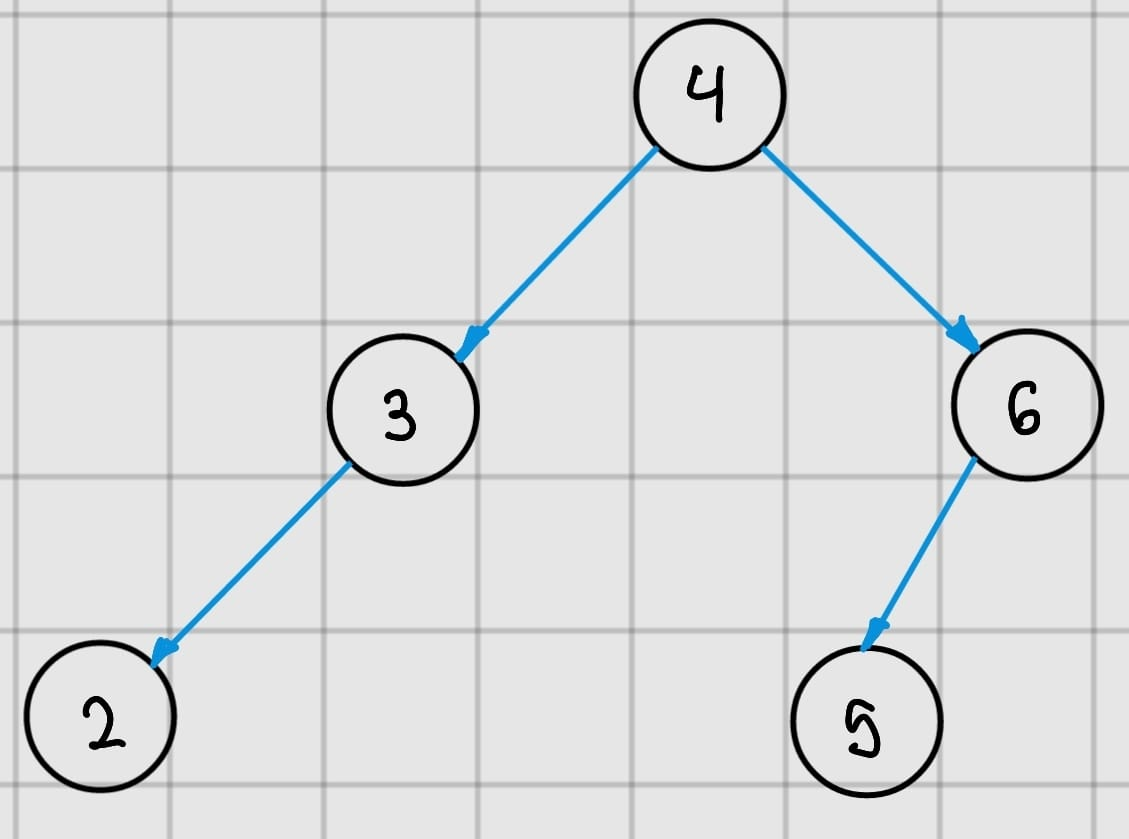
\includegraphics[width=\linewidth]{assets/abb_haskell.jpg}
\end{minipage}\]

\end{document} 
